\chapter{Neuronales Netz}
\label{ch:neuronalesNetz}
Im folgenden Kapitel wird das Training eines neuronalen Netzes eingeleitet und überwacht. Die dafür benötigten Testdaten
werden strukturier, aufbereitet und anschließend zum Training vorbereitet und verwendet. Das trainierte Modell soll für
später folgende Anwendungen aufrufbar sein um Vorhersagen in Echtzeit zu tätigen.

Sowohl über ein Webdienst als auch über ein Deployment soll das trainierte Modell Erreichbar sein. Dafür werden, wie in
Abbildung~\ref{fig:schematische_architektur} auf Seite~\pageref{fig:schematische_architektur} zu sehen, zwei
unterschiedliche Anwendungen angelegt und eingerichtet.

Die Kommunikation mit den beiden Anwendungen geschieht über den Austausch von JSON-Objekten über REST-Schnittstellen.
Damit die Kommunikation zentral gesteuert sowie einfach wartbar ist, soll ein API-Gateway zwischen Anwendung und den
beiden Deployments für den nötigen Komfort sorgen.

Der einzurichtende API-Gateway-Service \textit{API Connect} soll über zwei verwaltete Endpunkte verfügen. Einer steht
für die Kommunikation mit dem Webdienst. Der Andere für die Kommunikation mit dem Deployment.

Ziel der Architektur ist die Bereitstellung eines trainierten Modells, welches aus einem neuronalen Netz hervorgeht. Die
Architektur soll so aufgebaut werden, dass sie im Weiteren gut Wartbar und vor allem Erweiterbar ist.

Außerdem soll ein Test ergeben, ob das selbe trainierte Modell auch unter zwei verschiedenen Implementierungen zum
gleichen Ergebnis für Vorhersagen mit den gleichen Eingabeparametern kommt und warum es eventuell Abweichungen geben
kann.\\

\begin{figure}[h]
    \centering
    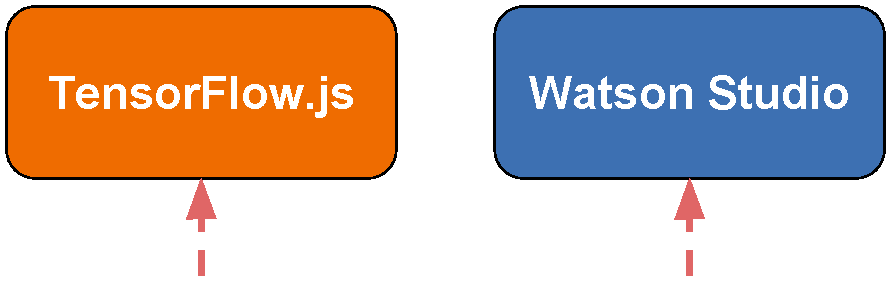
\includegraphics[scale=0.5]{images/kapitel_3/architektur_schematisch.pdf}
    \caption{Schematische Darstellung der Architektur}
    \label{fig:schematische_architektur}
\end{figure}